\documentclass{article}

\usepackage{circuitikz} %Für die Schaltpläne
\usepackage[T1]{fontenc} 
\usepackage[utf8]{inputenc}
\usepackage{amsmath}
\usepackage{amssymb}
\usepackage{fancyhdr}
\usepackage{graphicx}
\usepackage{hyperref}
\usepackage{subcaption}
\usepackage{tikz}
\usepackage{../assets/scripts/tex/color-env}
\usepackage[ngerman]{babel}



    \usetikzlibrary{arrows}
    \usetikzlibrary{arrows.meta,topaths}
    \usetikzlibrary{bending}
    \usetikzlibrary{calc}
\title{Elektrotechnik 1 Praktikum 1}


\usepackage[
  includehead,
  headheight = 17mm,
  footskip = \dimexpr\headsep+\ht\strutbox\relax,
  tmargin = 0mm,
  bmargin = \dimexpr17mm+2\ht\strutbox\relax,
]{geometry}

\usepackage{anyfontsize}

\usepackage{xcolor}

\definecolor{DarkGreenBlue}{HTML}{264653}
\definecolor{LightGreenBlue}{HTML}{2A9D8F}
\definecolor{LightOrange}{HTML}{E9C46A}
\definecolor{DarkOrange}{HTML}{F4A261}
\definecolor{RedOrange}{HTML}{E76F51}
\definecolor{BrightRed}{HTML}{D62828}
\definecolor{DeepBlue}{HTML}{003049}



\pagestyle{fancy}
\fancyhead[L]{\leftmark}
\fancyhead[R]{}
\fancyfoot[L]{}
\fancyfoot[C]{\thepage}
\fancyfoot[R]{
\includegraphics[scale=0.2]{../assets/images/haw.jpg}}
\renewcommand\headrulewidth{0.5pt}


\begin{document}



\begin{tikzpicture}[overlay,remember picture]
  \thispagestyle{empty}
  \fill[black!2] (current page.south west) rectangle (current page.north east);

  \begin{scope}[transform canvas ={rotate around ={45:($(current page.north west)+(-.5,-6)$)}}]

    \shade[rounded corners=18pt, left color=DarkGreenBlue, right color=LightGreenBlue] ($(current page.north west)+(-.5,-6)$) rectangle ++(9,1.5);

  \end{scope}

  \begin{scope}[transform canvas ={rotate around ={45:($(current page.north west)+(.5,-10)$)}}]

    \shade[rounded corners=18pt, left color=LightOrange,right color=DarkOrange] ($(current page.north west)+(0.5,-10)$) rectangle ++(15,1.5);

  \end{scope}

  \begin{scope}[transform canvas ={rotate around ={45:($(current page.north west)+(0.5,-10)$)}}]

    \shade[rounded corners=8pt, right color=DarkOrange, left color=LightOrange] ($(current page.north west)+(1.5,-9.55)$) rectangle ++(7,.6);

  \end{scope}

  \begin{scope}[transform canvas ={rotate around ={45:($(current page.north)+(-1.5,-3)$)}}]

    \shade[rounded corners=12pt, left color=DeepBlue!80, right color=DeepBlue!60] ($(current page.north)+(-1.5,-3)$) rectangle ++(9,0.8);

  \end{scope}

  \begin{scope}[transform canvas ={rotate around ={45:($(current page.north)+(-3,-8)$)}}]

    \shade[rounded corners=28pt, left color=BrightRed, right color=BrightRed!80] ($(current page.north)+(-3,-8)$) rectangle ++(15,1.8);

  \end{scope}

  \begin{scope}[transform canvas ={rotate around ={45:($(current page.north west)+(4,-15.5)$)}}]

    \shade[rounded corners=25pt, left color=RedOrange, right color=DarkOrange] ($(current page.north west)+(4,-15.5)$) rectangle ++(30,1.8);

  \end{scope}

  \begin{scope}[transform canvas ={rotate around ={45:($(current page.north west)+(13,-10)$)}},]

    \shade[rounded corners=22pt, left color=DeepBlue,right color=DarkGreenBlue] ($(current page.north west)+(13,-10)$) rectangle ++(15,1.5);

  \end{scope}

  \begin{scope}[transform canvas ={rotate around ={45:($(current page.north west)+(18,-8)$)}},]

    \shade[rounded corners=8pt, left color=DarkOrange] ($(current page.north west)+(18,-8)$) rectangle ++(15,0.6);

  \end{scope}

  \begin{scope}[transform canvas ={rotate around ={45:($(current page.north west)+(19,-5.65)$)}},]

    \shade[rounded corners=12pt, left color=RedOrange] ($(current page.north west)+(19,-5.65)$) rectangle ++(15,0.8);

  \end{scope}

  \begin{scope}[transform canvas ={rotate around ={45:($(current page.north west)+(20,-9)$)}}]

    \shade[rounded corners=20pt, left color=BrightRed, right color=BrightRed!80] ($(current page.north west)+(20,-9)$) rectangle ++(14,1.2);

  \end{scope}

  \draw[ultra thick,gray] ($(current page.center)+(5,2)$) -- ++(0,-3cm) node[midway,left=0.25cm,text width=5cm,align=right,black!75]{{\fontsize{25}{30} \selectfont \bf Elektronik 1\\[10pt] Praktikum 3}} node[midway,right=0.25cm,text width=6cm,align=left,orange]{{\fontsize{70}{86} \selectfont 2020}};

  \node at ($(current page.center)+(0,-4)$) {{\fontsize{60}{72} \selectfont Bipolar Transistor}};

  \node[text width=8cm,align=center] at ($(current page.center)+(0,-6.5)$) {{\fontsize{16}{20} \selectfont \textcolor{orange}{ \bf \today}} \\[3pt] Florian Tietjen\\[3pt] Eric Antosch};

\end{tikzpicture}
\newpage
\thispagestyle{empty}

\tableofcontents


\newpage


\section{Kennlinie eines npn-Transistors}
\begin{task}
  TBei dieser Aufgabe sollen die Kennlinienfelder eines BC546A npn-Transistors mithilfe von LTSpice simuliert und analysiert werden. Dazu sollen bestimmte Kenndaten aus den Kennlinienfeldern rausgelesen werden.
\end{task}

\begin{figure}[h]
  \centering
  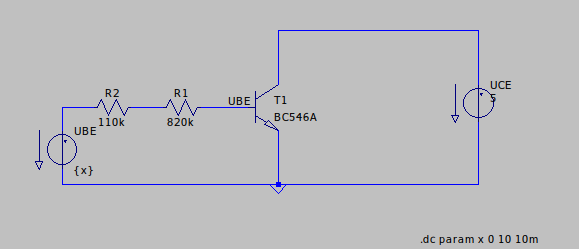
\includegraphics[scale=0.76]{../assets/images/EL1P3/Schaltplan1.png}
  \caption{Schaltplan zur Messung der Kennlinienfelder}
  \label{fig:schalt1}
\end{figure}

\subsection{Ausgangskennlinie}
\label{sec:ausgangskennlinie}

\subsubsection{Vorbereitung}


Wir wollen zunächst das Ausgangskennlinienfeld des Transistors bestimmen. Dazu messen wir $I_{C} = 0...2mA$ und $U_{CE} = 0...10V$ für mindestens 5 verschiedene Basisströme und tragen diese
in LTSpice ab. Für die Basisströme benutzen wir eine variable Spannungsquelle mit einem hochohmigen Vorwiderstand aus der E24-Reihe. Wir wissen aus dem Datenblatt des BC546A, dass die Stromverstärkung bei ca. $B=200$ liegt, wir rechnen also:
\begin{equation}
  \label{eq:1}
  I_{B} = \frac{I_{CE}}{B} = \frac{2mA}{200} = 10\mu A.
\end{equation}
Wir wählen nun eine Spannungsquelle mit einem Maximum von 10V. Um das Maximum von $I_{B} = 10\mu A$ zu bekommen, wollen wir nun den Vorwiderstand unter Berücksichtigung von $U_{BE} = 0,7V$ bestimmen:
\begin{equation}
  \label{eq:2}
  R_{V} = \frac{U_{0}-U_{BE}}{I_{B}} = \frac{10V-0,7V}{10\mu A} = 930k\Omega.
\end{equation}

\subsubsection{Durchführung}
Wir setzen den Wert von $R_{V} = 930k\Omega$ aus den Widerständen $R_{V1} = 110k\Omega$ und $R_{V2} = 820k\Omega$ zusammen (siehe (\ref{fig:schalt1})). Wir variieren nun mit DC-Sweep den Wert von $UCE$ zwischen $0V-10V$ in einem linearen Inkrement von $\Delta I = 10\mu A$. Den Basisstrom nehmen wir für die Werte 2V, 4V, 5V, 6V, 8V und 10V auf und stellen den in einem Kennlinienfeld dar.

\begin{figure}[h]
  \centering
  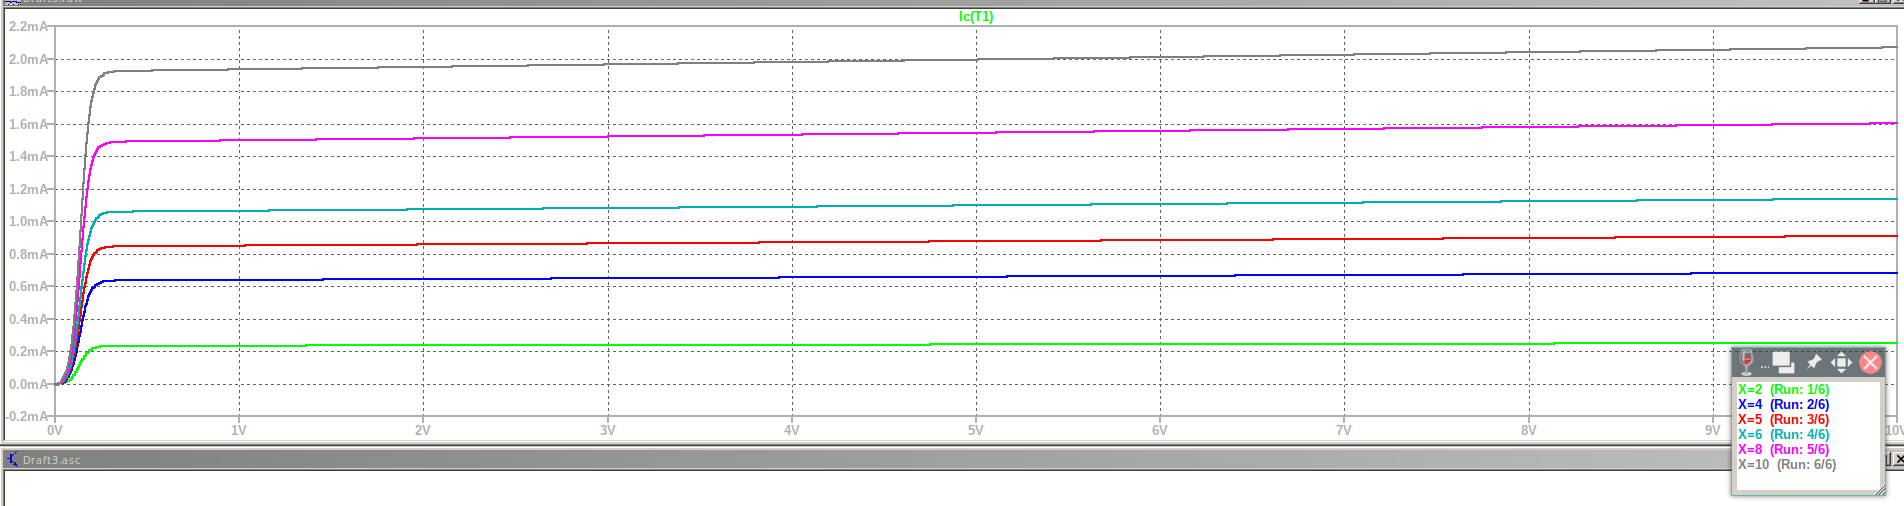
\includegraphics[width=\textwidth]{../assets/images/EL1P3/ausgangskennlinie.png}
  \caption{Ausgangskennlinie der Messschaltung mit verschiedenen Basisströmen}
  \label{fig:ausgang}
\end{figure}

\subsubsection{Auswertung}

Wir lesen nun aus der Abbildung (\ref{fig:ausgang}) den Wert von $I_{C} = 2mA$ an der Stelle $U_{CE} = 5V$ und einem Basisstrom $I_{B} = 10\mu A$. Aus
\begin{equation}
  \label{eq:3}
  B = \frac{I_{C}}{I_{B}} = \frac{2mA}{10\mu A} = 200.
\end{equation}

folgt, dass unsere ermittelte Stromverstärkung der erwarteten Stromverstärkung aus dem Datenblatt bzw. der Vorbereitung enspricht. Um nun die Early-Spannung zu ermitteln, nutzen wir die Cursorfunktion von LTSpice und legen ein Steigungsdreieck an eine der Kennlinien an (wir haben uns für $I_{B} = 2\mu A$ entschieden). Zwischen $U_{CE} = 1V...2V$ ist eine Steigung von $m = 1,818\cdot 10^{-6}$ festzustellen. Von $f_{I_{B1}}(U_{CE}) = f_{2\mu A}(1V) = 233,1964\mu A$ ausgehend bestimmen wir nun den Schnittpunkt der angelegten Geraden mit der X-Achse im Negativen:
\begin{equation}
  \label{eq:4}
  0 = 1,818\cdot 10^{-6}\cdot x + 231,3784\mu A
\end{equation}
Nach dem wir nun die Gleichung nach $x$ auflösen, erhalten wir den Wert $x = -127,27$. Dies ist der Wert der Early-Spannung $U_{A} = -127,27V$.
\newpage

\subsection{Übertragungskennlinie}
\label{sec:ubertr}

Als nächstes wollen wir das Übertragungskennliniefeld des Transistors messen. Wir halten nun die Spannungs $U_{CE} = 5V$ fest und variieren nur noch den Basisstrom zwischen $I_{B} = 0...10\mu A$. Dabei bleibt die Messchaltung beinahe identisch.

\begin{figure}[h]
  \centering
  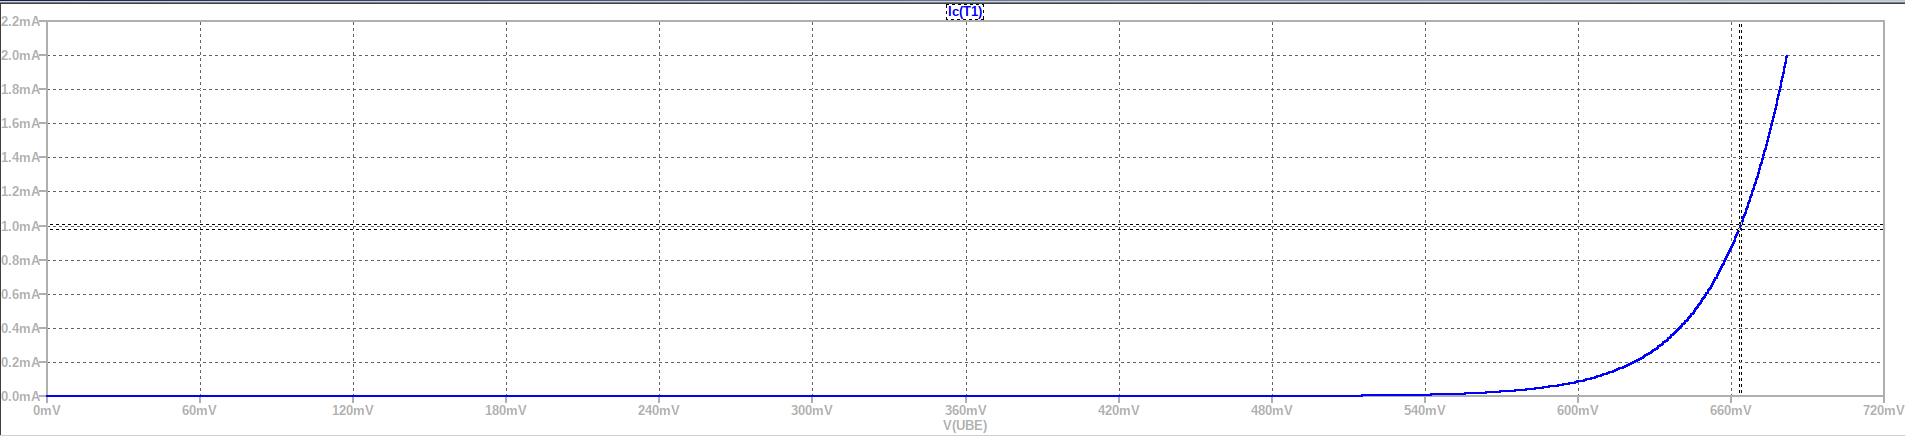
\includegraphics[width=\textwidth]{../assets/images/EL1P3/uebertragungskennlinie.png}
  \caption{Übertragungskennlinienfeld der Messchaltung}
  \label{fig:uebertragungskennlinie}
\end{figure}

\subsubsection{Auswertung}

Wir wollen nun die Steilheit an dem Punkt $I_{C} = 1mA$ bestimmen. Dazu legen wir mit der Cursorfunktion von LTSpice an den Punkt ein Steigungsdreieck an und lesen den gegebenen Wert ab. Es ergibt sich ein Wert von $r_{d} = 0,0383771\Omega$.

\newpage

\subsection{Steuerkennlinie}
\label{sec:steuerkennlinie}

Zum Schluss wollen wir nun auch die Steuerkennlinie betrachten. Dazu nutzen wir erneut die gleiche Schaltung wie in den letzten beiden Messungen, wobei wir nun $I_{B}$ gegen $I_{C}$ abtragen. Auch hier halten wir $U_{CE} = 5V$ fest, während $I_{B} = 0...10\mu A$ variiert. Das Ergebnis halten wir in einem Plot fest, der eine beinahe lineare Auslenkung besitzt.

\begin{figure}[h]
  \centering
  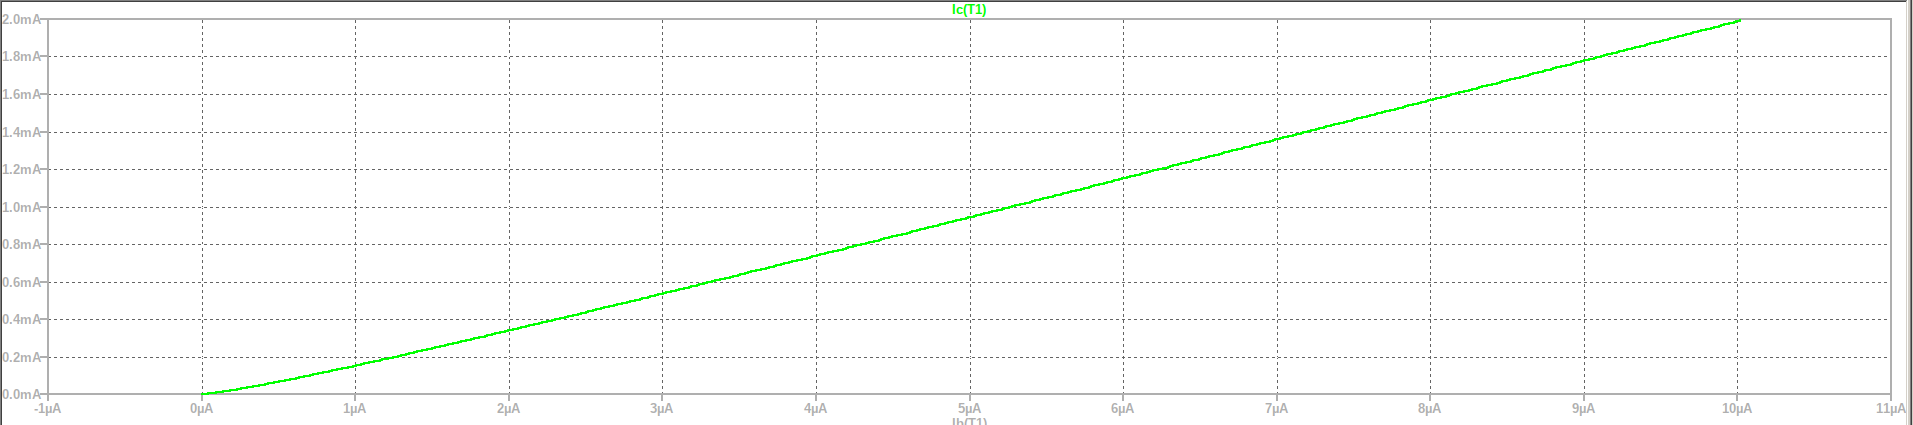
\includegraphics[width=\textwidth]{../assets/images/EL1P3/steuerkennlinie.png}
  \caption{Steuerkennlinie des Messschaltung}
  \label{fig:steuer}
\end{figure}

\section{Durchlasskennlinien der Siliziumdiode in halblogarithmischer Darstellung}
\begin{task}
  TIn diesem Versuch wollen wir erneut die Kennlinie der 1N4148 Siliziumdiode aufnehmen, wobei wir sowohl mehr Messpunkte als auch 
  eine halblogarithmische Darstellung wählen.
\end{task}

\begin{figure}[h]
  \begin{center}
    \begin{circuitikz}[european]
      \draw (0,0) to[vsource, l=$U_0$] (0,4) to[diode, l_=$D$] (4,4) to[R, l_=$R_v$] (4,0);
      \draw (0,0) to[ammeter] (4,0);
      \draw (1,4) to[short, *-] (1,5) to[voltmeter, l=$U_x$] (3,5) to[short, -*] (3,4);
    \end{circuitikz}
    \caption{Aufbauzeichnung der Messung mithilfe des MetraHit Tech Multimeter}
  \end{center}
\end{figure}

\begin{devlist}
  T\begin{itemize}
    \item Multimeter MetraHit X-TRA
    \item Gleichstromgenerator
    \item 1N4148 Siliziumdiode
  \end{itemize}
\end{devlist}
\newpage
\subsection{Vorbereitung}

\begin{figure}[h]
  \centering
  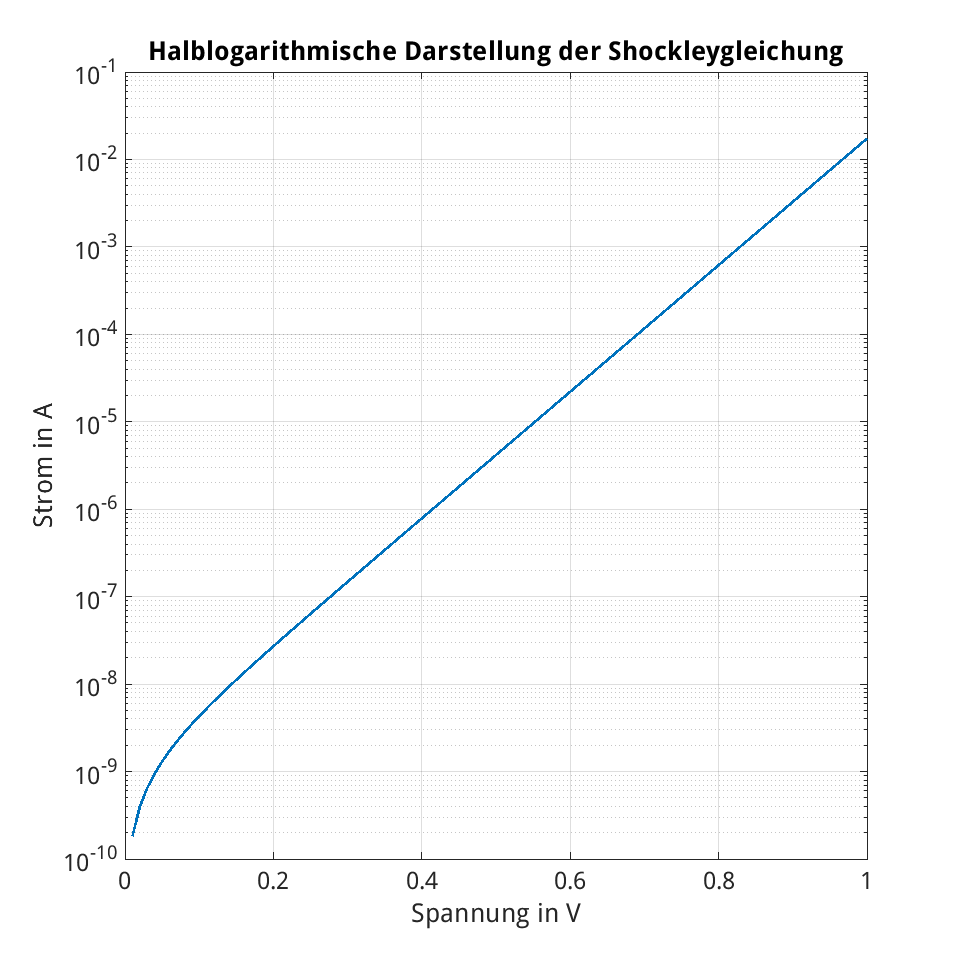
\includegraphics[scale=0.4]{../assets/images/EL1P2/VorbereitungSemilogDiode2.png}
  \caption{Semilogarithmische Darstellung der Shockleygleichung mit Matlab}
  \label{fig:vsemilog}
\end{figure}

Mithilfe von Matlab und der Shockleygleichung lässt sich eine halblogarithmische Darstellung der Diodenkennlinie erstellen, die man hier als stark linear erkennen kann.

\subsection{Versuchsdurchführung}

Wir lassen die Schaltung aus Aufgabe 1 weitesgehend aufgebaut und legen jetzt an die entsprechenden Stellen Multimeter(MetraHit Tech) an.

\begin{table}[h]
  \begin{center}
\begin{tabular}{|c|c|}
  \hline
  $I_{f}$ & $U_{f}$  \\
  \hline
  $10\mu A$ & 0,396V\\
  \hline
  $20\mu A$ & 0,433V\\
  \hline
  $50\mu A$ & 0,4761V\\
  \hline
  $100\mu A$ & 0,5079V\\
  \hline
  $200\mu A$ & 0,5418V\\
  \hline
  $500\mu A$ & 0,5873\\
  \hline
  $1mA$ &
          0,6219V\\
  \hline
  $2mA$ & 0,6551V\\
  \hline
  $5mA$ & 0,7018V\\
  \hline
  $10mA$ & 0,7393V\\
  \hline
\end{tabular}
\caption{Messwerte, die mit dem Multimeter aufgenommen wurden in tabellarischer Form}
\end{center}
\end{table}

\begin{figure}[h]
  \begin{center}
    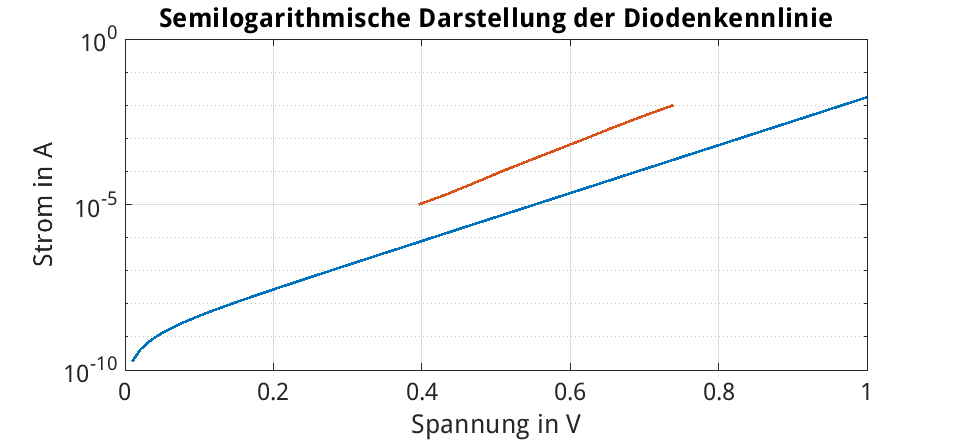
\includegraphics[scale=0.6]{../assets/images/EL1P2/SemilogDiodeVergleich.png}
    \caption{Semilogarithmische Darstellung der Diodenkennlinie mit Matlab}
  \end{center}
\end{figure}

Hier ist nun die Diodenkennlinie aus der Vorbereitung mit der neuen Kennlinie aus den Messwerten (orange) dargestellt.
\newpage
\subsection{Auswertung}

Es ist interessant, dass sowohl die Diodengleichung als auch die Messergebnisse zu sehr ähnlichen Grafiken führen, die nahezu linear sind. Dies ist jedoch nicht sehr verwunderlich, da in der Shockleygleichung auch ein Term mit $e$ vorkommt. Der Versatz, der sich zwischen beiden Kennlinie ergibt, kann aus vielen Faktoren entstanden seien, die aus der empfindlichen Art der Diode entstehen können. Dadurch, dass Halbleiterelemente zudem sehr temperaturabhängig sind, kann auch die Raumtemperatur des Labors eine Rollen spielen.

\newpage

\section{Einweggleichrichterschaltung}
\begin{task}
  TIn diesem Versuch wollen wir die Eigenschaften einer Einweggleichrichterschaltung mithilfe der uns 
  vermittelten Methoden analysieren und auswerten.
\end{task}

\begin{devlist}
  T\begin{itemize}
    \item Oszilloskop
    \item Funktionsgenerator
    \item Multimeter
    \item Lastwiderstand
    \item Kondensator
    \item 1N4148 Siliziumdiode
  \end{itemize}
\end{devlist}

\begin{figure}[h]
  \begin{center}
    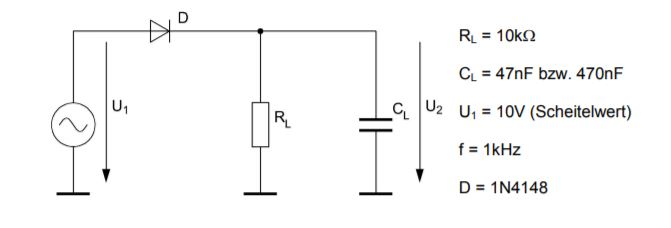
\includegraphics{../assets/images/EL1P2/aufgabe 3 schaltung.JPG}
    \caption{Einweggleichrichterschaltung mit Glättungskondensator}
  \end{center}
\end{figure}

\subsection{Darstellung der Zeitverläufe von $U_1$ und $U_2$}

\begin{figure}[h]
  \begin{center}
    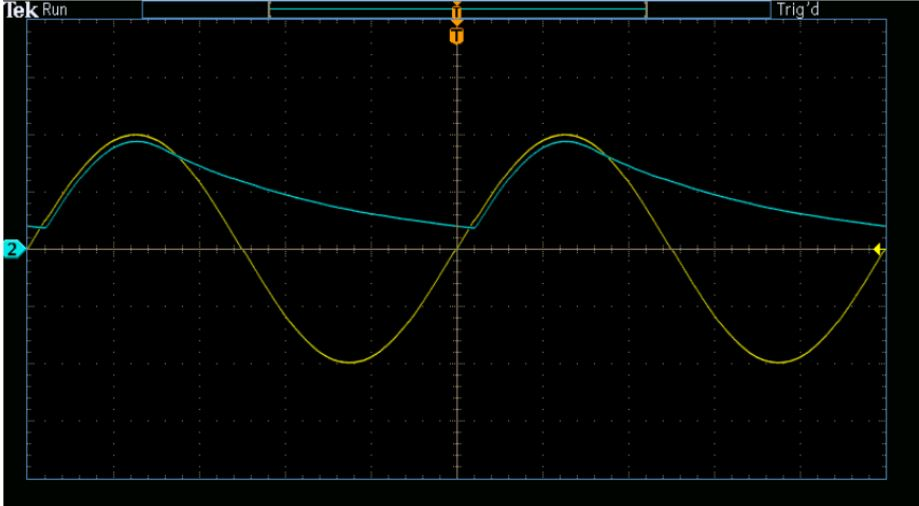
\includegraphics[scale=0.6]{../assets/images/EL1P2/aufgabe 3 47n.JPG}
    \caption{Spannungsverlauf bei $C_L$ = 47nF}
  \end{center}
\end{figure}

\begin{figure}[h]
  \begin{center}
    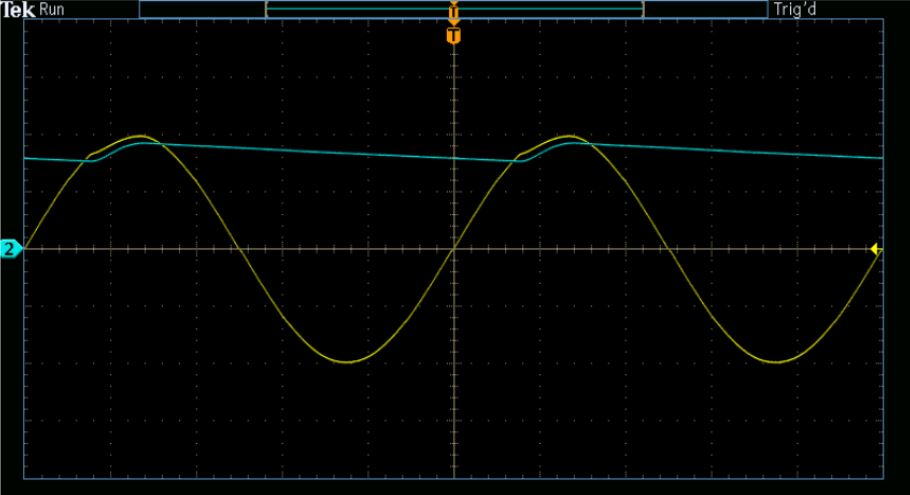
\includegraphics[scale=0.6]{../assets/images/EL1P2/aufgabe 3 470n.JPG}
    \caption{Spannungsverlauf bei $C_L$ = 470nF}
  \end{center}
\end{figure}

\newpage

\subsection{Messung von Gesamteffektivwert, Wechseleffektivwert und des Mittelwertes von $U_1$ und $U_2$}

\begin{table}[h]
  \begin{center}
\begin{tabular}{|c|c|c|}
  \hline
  & $U_{1}$ & $U_{2}$  \\
  \hline
  U\raisebox{-0.9ex}{\~{}} & 7,053V & 2,42V\\
  \hline
  $U_{TRMS}$ & 7,053V&5,681V\\
  \hline
  $U_{DC}$ & -0.5V&5,151V\\
  \hline
\end{tabular}
\caption{Messwerte bei $C_L$ = 47nF}
\end{center}
\end{table}

\begin{table}[h]
  \begin{center}
\begin{tabular}{|c|c|c|}
  \hline
  & $U_{1}$ & $U_{2}$  \\
  \hline
  U\raisebox{-0.9ex}{\~{}} & 7,053V & 1,756V\\
  \hline
  $U_{TRMS}$ & 7,053V & 6,63V\\
  \hline
  $U_{DC}$ & -0.5V  & 6,414\\
  \hline
\end{tabular}
\caption{Messwerte bei $C_L$ = 470nF}
\end{center}
\end{table}

\subsection{Welligkeit von $U_2$}

Die Welligkeit ist definiert als das Verhältnis vom Effektivwert des Wechselanteils U\raisebox{-0.9ex}{\~{}} zum Betrag des Gleichanteils $U_{DC}$:

\begin{align*}
  r_u = \frac{U\raisebox{-0.9ex}{\~{}}}{|U_{DC}|}
\end{align*}

Für $C_L$ = 47nF gilt ergibt sich folgende Welligkeit der Spannung:
\begin{align*}
  r_u = \frac{2,42V}{5,151V} = 0,47
\end{align*}
Und für $C_L$ = 470nF:
\begin{align*}
  r_u = \frac{1,756V}{6,414V} = 0,27
\end{align*}

Je kleiner die Welligkeit, desto stärker die Glättung des Signals. Diese Glättung ist abhängig von der Kapazität des Kondensators, je größer sie ist, desto besser die Glättung und kleiner die Welligkeit.
\\ In der Nachbereitung ist aufgefallen, dass die gemessenen Spannungen bei $U_2$ für $C_L$ = 470nF zu gering sind. Dies kann an der Auswahl eines falschen Kondensators liegen.
Dennoch lässt sich trotzdem erkennen, dass die Werte größer sind als bei der kleineren Kapazität.

\section{Zweiweggleichrichterschaltung}

\begin{task}
  TIn dem letzten Versuch wollen wir nun die Eigenschaften einer Zweiweggleichrichterschaltung mithilfe der uns vermittelten
  Methoden analysieren und auswerten.
\end{task}

\begin{devlist}
  T\begin{itemize}
    \item Oszilloskop
    \item Funktionsgenerator
    \item Multimeter
    \item Lastwiderstand
    \item Kondensator
    \item 1N4148 Siliziumdiode
  \end{itemize}
\end{devlist}

\begin{figure}[h]
  \begin{center}
    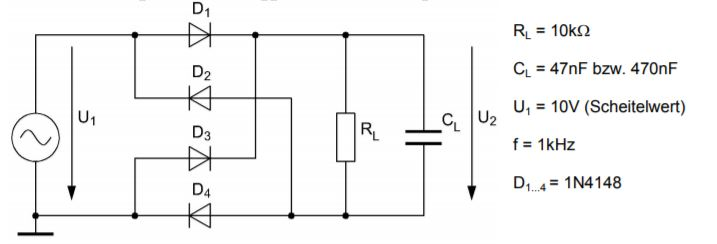
\includegraphics{../assets/images/EL1P2/aufgabe 4 schaltung.JPG}
    \caption{Zweiweggleichrichterschaltung}
  \end{center}
\end{figure}

\newpage

\subsection{Darstellung der Zeitverläufe von $U_1$ und $U_2$}

\begin{figure}[h]
  \begin{center}
    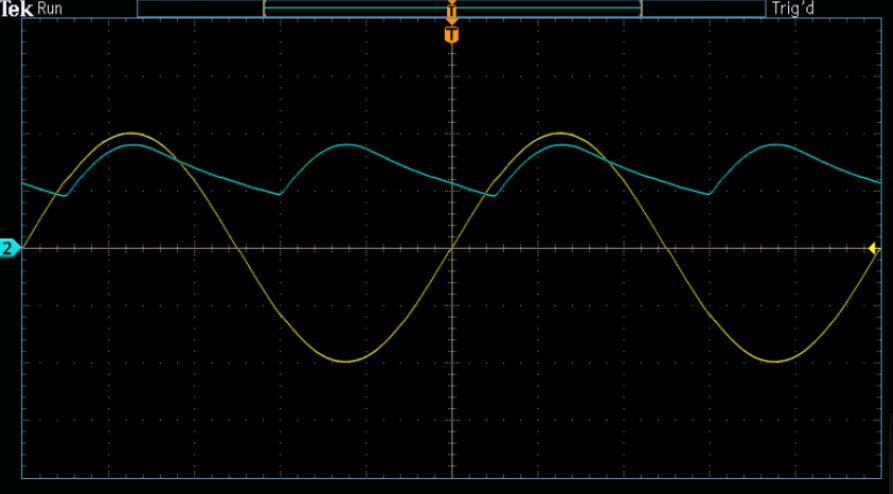
\includegraphics[scale=0.7]{../assets/images/EL1P2/aufgabe 4 47n.JPG}
    \caption{Spannungsverlauf bei $C_L$ = 47nF}
  \end{center}
\end{figure}

\begin{figure}[h]
  \begin{center}
    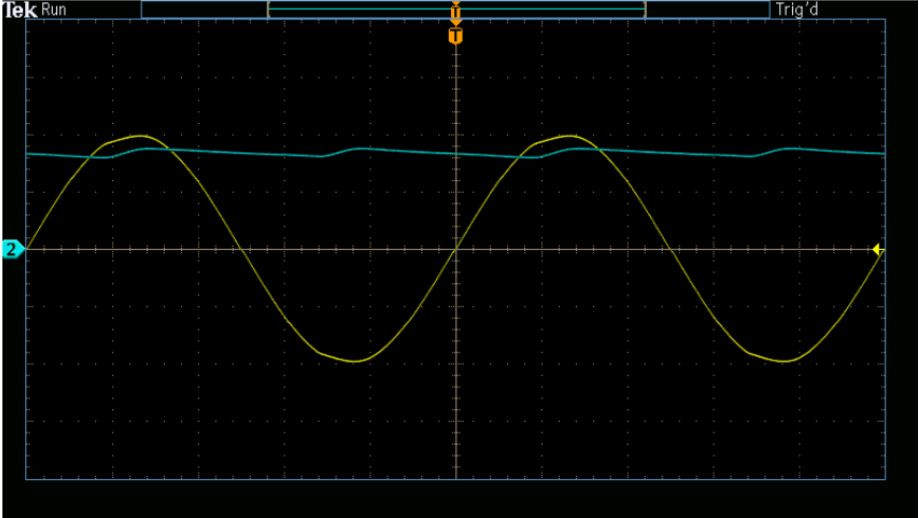
\includegraphics[scale=0.6]{../assets/images/EL1P2/aufgabe 4 470n.JPG}
    \caption{Spannungsverlauf bei $C_L$ = 470nF}
  \end{center}
\end{figure} 

\newpage

\subsection{Messung von Gesamteffektivwert, Wechseleffektivwert und des Mittelwertes von $U_1$ und $U_2$}

\begin{table}[h]
  \begin{center}
\begin{tabular}{|c|c|c|}
  \hline
  & $U_{1}$ & $U_{2}$  \\
  \hline
  U\raisebox{-0.9ex}{\~{}} & 7,012V & 1,441V\\
  \hline
  $U_{TRMS}$ & 7,012V&7,42V\\
  \hline
  $U_{DC}$ & -0.53V&7,382V\\
  \hline
\end{tabular}
\caption{Messwerte bei $C_L$ = 47nF}
\end{center}
\end{table}

\begin{table}[h]
  \begin{center}
\begin{tabular}{|c|c|c|}
  \hline
  & $U_{1}$ & $U_{2}$  \\
  \hline
  U\raisebox{-0.9ex}{\~{}} & 7,012V & 0,21V\\
  \hline
  $U_{TRMS}$ & 7,012V & 8,172V\\
  \hline
  $U_{DC}$ & -0.53V  & 8,172V\\
  \hline
\end{tabular}
\caption{Messwerte bei $C_L$ = 470nF}
\end{center}
\end{table}

\subsection{Welligkeit von $U_2$}

Ganz analog zu Versuch 3 wird nun wieder die Welligkeit bestimmt:

\begin{align*}
  r_u = \frac{U\raisebox{-0.9ex}{\~{}}}{|U_{DC}|}
\end{align*}

Für $C_L$ = 47nF gilt ergibt sich folgende Welligkeit der Spannung:
\begin{align*}
  r_u = \frac{1,441V}{7,382} = 0,2
\end{align*}
Und für $C_L$ = 470nF:
\begin{align*}
  r_u = \frac{0,21}{8,172} = 0,026
\end{align*}

Im Vergleich zur Einweggleichrichterschaltung ergibt sich eine noch geringere Welligkeit und damit ein noch besseres gleichgerichtetes Signal.
Durch die Verschaltung von vier Dioden kommt es zu keinem Zeitpunkt zu einer kompletten Sperrung der Quellspannung $U_1$.

\end{document}
